%%%%%%%%%%%%%%%%%%%%%%%%%%%%%%%%%%%%%%%%%%%%%%%%%%%%%%%%%%%%%%%%%%%%%%%%%%%%%%%%%%
\begin{frame}[fragile]\frametitle{}
\begin{center}
{\Large Database}
\end{center}
\end{frame}


%%%%%%%%%%%%%%%%%%%%%%%%%%%%%%%%%%%%%%%%%%%%%%%%%%%%%%%%%%%%%%%%%%%%%%%%%%%%%%%%%%
\begin{frame}\frametitle{Background}

\begin{itemize}
\item A Database is a place to store application data, to process and query, etc

\item Relational databases (SQL) store data in tables. Strict schema.
\item Document?key-value databases (no-SQL) store data in dictionaries/json. Flexi schema.
\item A Graph Database is where data is stored in graph data structure ie nodes and edges.
\end{itemize}

\begin{center}
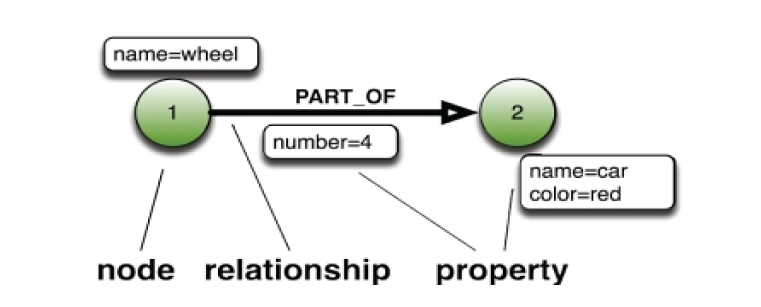
\includegraphics[width=0.5\linewidth,keepaspectratio]{neo4j29}
\end{center}	

{\tiny (Ref: Neo4j (Graph Database) Crash Course - Laith Academy)}
\end{frame}

%%%%%%%%%%%%%%%%%%%%%%%%%%%%%%%%%%%%%%%%%%%%%%%%%%%%%%%%%%%%%%%%%%%%%%%%%%%%%%%%%%
\begin{frame}\frametitle{Example}


\begin{center}
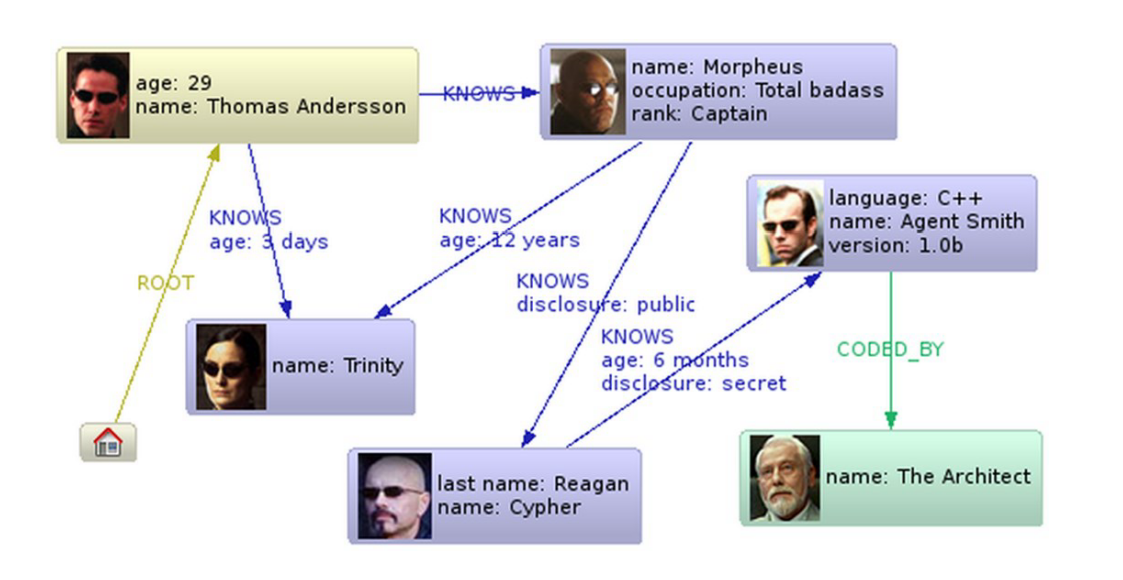
\includegraphics[width=\linewidth,keepaspectratio]{neo4j30}
\end{center}	

{\tiny (Ref: CIS 6930 - Advanced Databases - Neo4j )}
\end{frame}

%%%%%%%%%%%%%%%%%%%%%%%%%%%%%%%%%%%%%%%%%%%%%%%%%%%%%%%%%%%
\begin{frame}[fragile]\frametitle{Relational Database}
SQL

\begin{center}
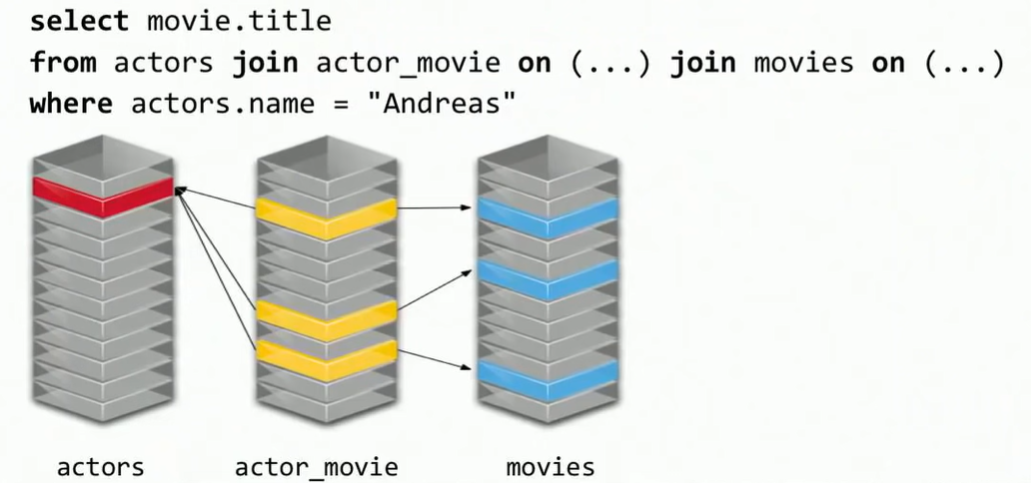
\includegraphics[width=\linewidth,keepaspectratio]{neo4j17}
\end{center}	    

{\tiny (Ref: Introduction to Neo4j and Graph Databases
 - M David Allen)}

\end{frame}

%%%%%%%%%%%%%%%%%%%%%%%%%%%%%%%%%%%%%%%%%%%%%%%%%%%%%%%%%%%
\begin{frame}[fragile]\frametitle{Graph Database}
Cypher

\begin{center}
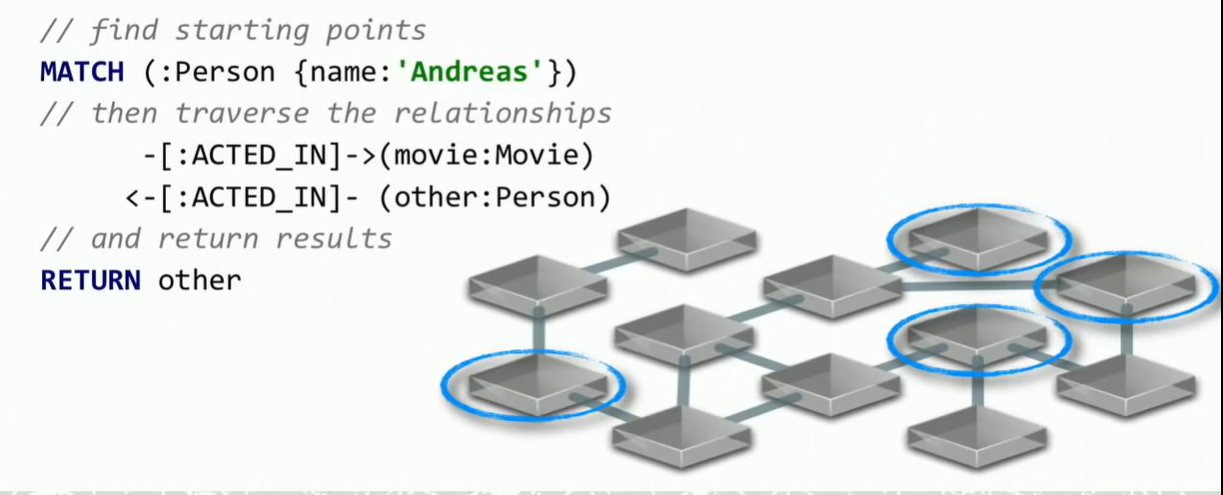
\includegraphics[width=\linewidth,keepaspectratio]{neo4j18}
\end{center}	    

{\tiny (Ref: Introduction to Neo4j and Graph Databases
 - M David Allen)}

\end{frame}

%%%%%%%%%%%%%%%%%%%%%%%%%%%%%%%%%%%%%%%%%%%%%%%%%%%%%%%%%%%%%%%%%%%%%%%%%%%%%%%%%%
\begin{frame}\frametitle{RDBMS}

\begin{itemize}
\item Cannot model or store data and relationships well, ie, without complexity
\item Performance degrades with umber and levels of relationships and database size
\item Query complexity grows with the need for JOINs
\item Adding new types of data and relationships requires schema redesign
\item More difficult if that needs to be done real time.
\end{itemize}

{\tiny (Ref: Neo4j (Graph Database) Crash Course - Laith Academy)}
\end{frame}

%%%%%%%%%%%%%%%%%%%%%%%%%%%%%%%%%%%%%%%%%%%%%%%%%%%%%%%%%%%
\begin{frame}[fragile]\frametitle{Comparison}
Find all reports and how many people they manage upto 3 levels down.

\begin{center}
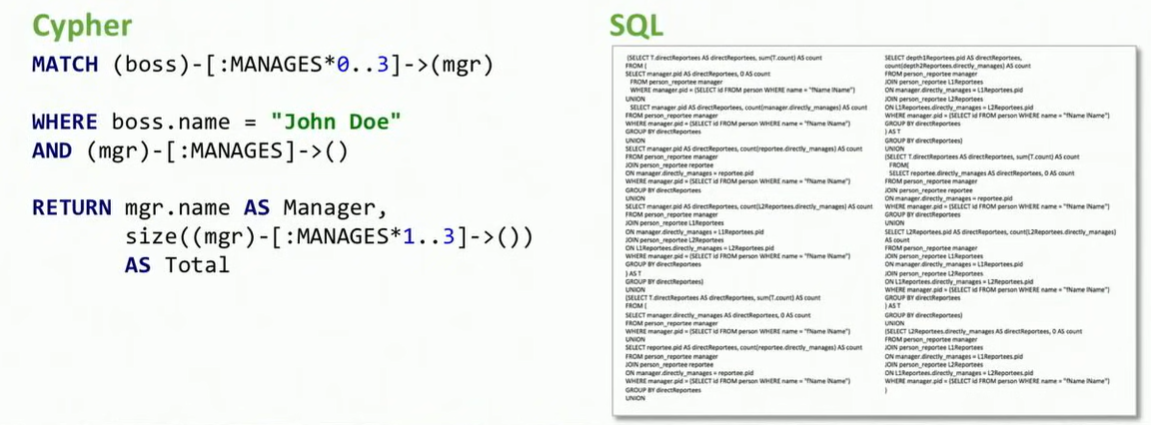
\includegraphics[width=\linewidth,keepaspectratio]{neo4j19}
\end{center}	    

{\tiny (Ref: Introduction to Neo4j and Graph Databases
 - M David Allen)}

\end{frame}

%%%%%%%%%%%%%%%%%%%%%%%%%%%%%%%%%%%%%%%%%%%%%%%%%%%%%%%%%%%
\begin{frame}[fragile]\frametitle{Same Data, Different Layout}
No more Tables, no more Doreign Keys, no more Joins
\begin{center}
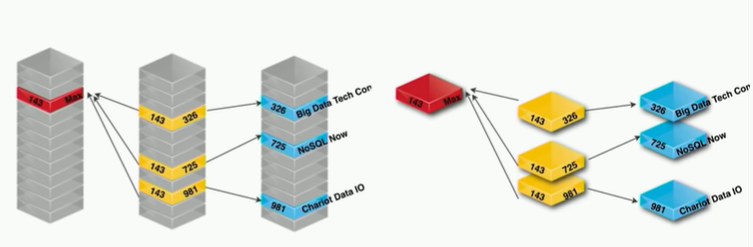
\includegraphics[width=\linewidth,keepaspectratio]{neo4j22}
\end{center}	    

{\tiny (Ref: Secret Sauce of Neo4j: Modeling and Querying Graphs
 - Max De Marzi )}

\end{frame}

%%%%%%%%%%%%%%%%%%%%%%%%%%%%%%%%%%%%%%%%%%%%%%%%%%%%%%%%%%%
\begin{frame}[fragile]\frametitle{Relational Databases cannot do Relationships}

\begin{center}
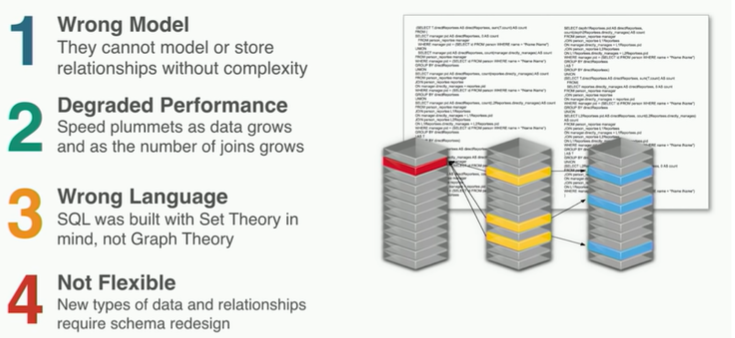
\includegraphics[width=\linewidth,keepaspectratio]{neo4j23}
\end{center}	    

{\tiny (Ref: Secret Sauce of Neo4j: Modeling and Querying Graphs
 - Max De Marzi )}

\end{frame}

%%%%%%%%%%%%%%%%%%%%%%%%%%%%%%%%%%%%%%%%%%%%%%%%%%%%%%%%%%%
\begin{frame}[fragile]\frametitle{No-SQL Databases cannot do Relationships}
Key-value pairs, no Joins, no connections

\begin{center}
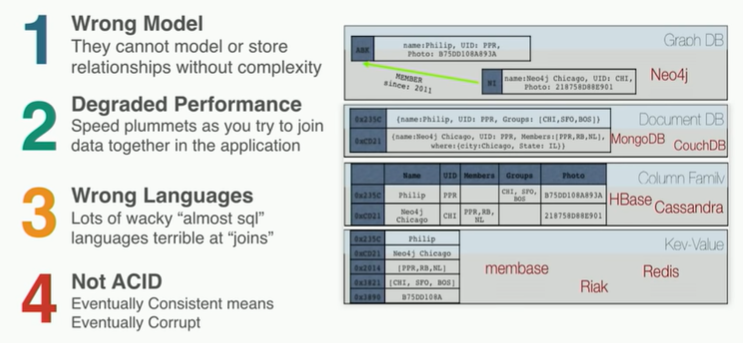
\includegraphics[width=\linewidth,keepaspectratio]{neo4j24}
\end{center}	    

{\tiny (Ref: Secret Sauce of Neo4j: Modeling and Querying Graphs
 - Max De Marzi )}

\end{frame}

%%%%%%%%%%%%%%%%%%%%%%%%%%%%%%%%%%%%%%%%%%%%%%%%%%%%%%%%%%%
\begin{frame}[fragile]\frametitle{Performance}
Remains steady as Database grows. Btw, suitable for graph like data only, and not like lists-queues like dataset where RDBM will work far better.

\begin{center}
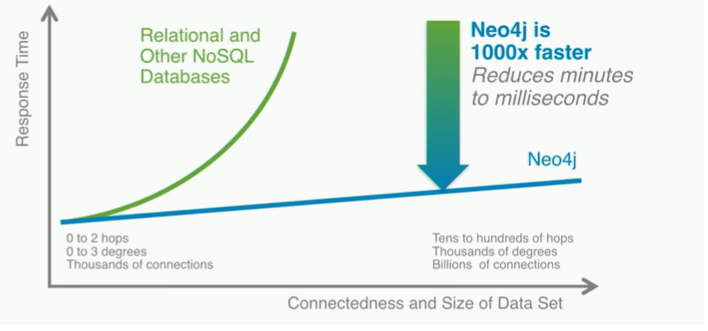
\includegraphics[width=\linewidth,keepaspectratio]{neo4j25}
\end{center}	    

{\tiny (Ref: Secret Sauce of Neo4j: Modeling and Querying Graphs
 - Max De Marzi )}

\end{frame}

%%%%%%%%%%%%%%%%%%%%%%%%%%%%%%%%%%%%%%%%%%%%%%%%%%%%%%%%%%%
\begin{frame}[fragile]\frametitle{Smells like a Graph?}

\begin{center}
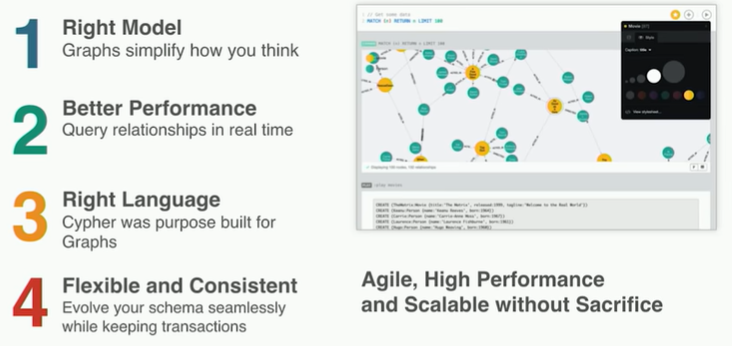
\includegraphics[width=\linewidth,keepaspectratio]{neo4j26}
\end{center}	    

{\tiny (Ref: Secret Sauce of Neo4j: Modeling and Querying Graphs
 - Max De Marzi )}

\end{frame}

%%%%%%%%%%%%%%%%%%%%%%%%%%%%%%%%%%%%%%%%%%%%%%%%%%%%%%%%%%%%%%%%%%%%%%%%%%%%%%%%%%
\begin{frame}\frametitle{Successful companies using graphs}


\begin{center}
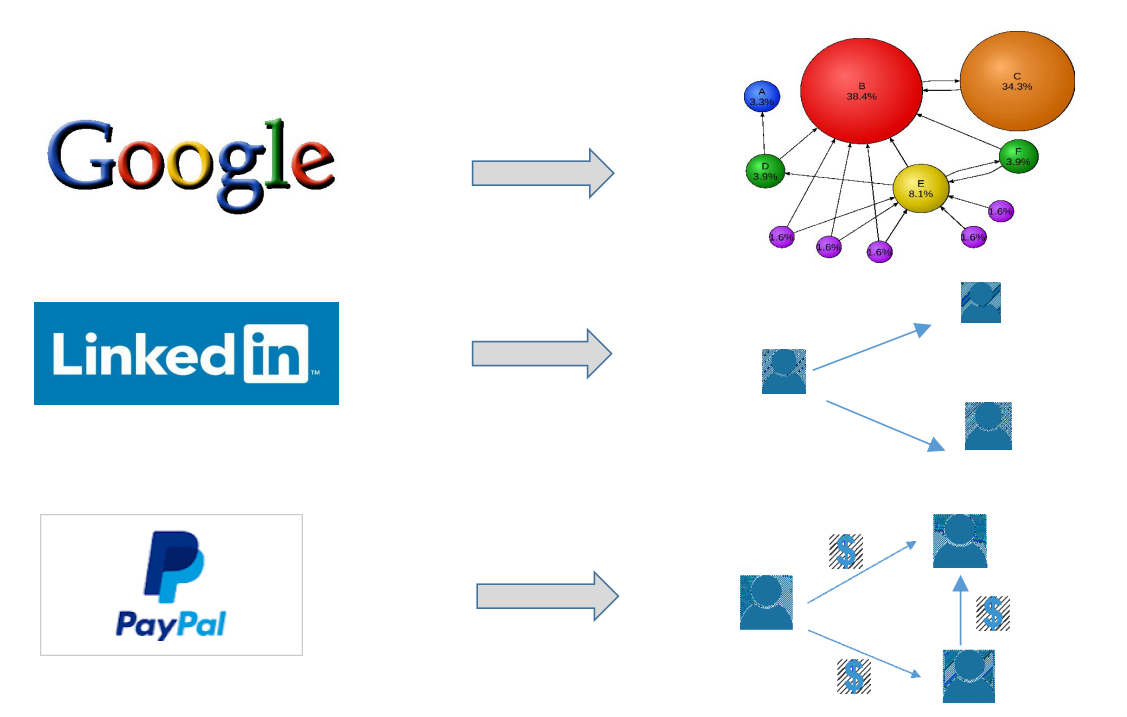
\includegraphics[width=0.8\linewidth,keepaspectratio]{neo4j31}
\end{center}	

{\tiny (Ref: CIS 6930 - Advanced Databases - Neo4j )}
\end{frame}

